\documentclass{sr}
\let\ifpdf\relax % http://tex.stackexchange.com/questions/11414/package-ifpdf-error

%\includeonly{ch01/ch01temp}

\makeindex
\pdfmapfile{=fullembed.map} % created by the script create_fullembed_file

\begin{document}

% Special Relativity
\thispagestyle{empty}
\raisebox{0mm}[0mm][0mm]{%
\parbox{8.5in}{
\vspace*{236mm}\hspace{-38.5mm}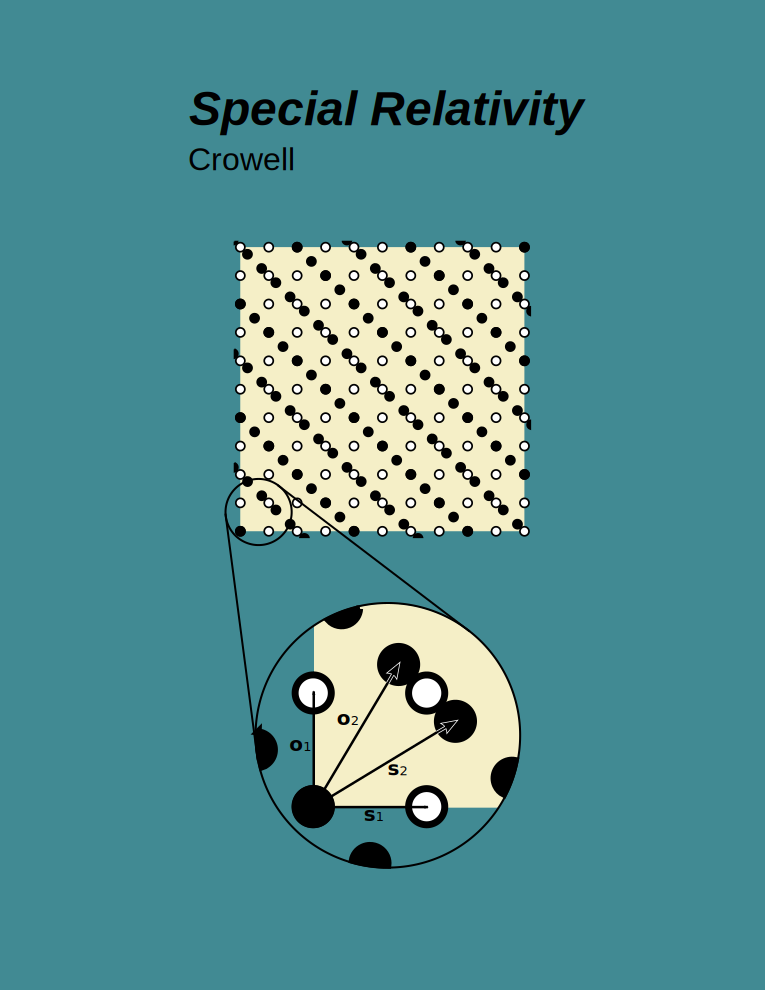
\includegraphics[width=\paperwidth]{cover/cover-for-pdf.png}\\
}
}%
\\


\cleardoublepage

\thispagestyle{empty}

\vspace{100mm}

{\sffamily

\noindent {\Huge Special Relativity}

\noindent Benjamin Crowell

\noindent www.lightandmatter.com

}


\thispagestyle{empty}

\vspace{100mm}

\noindent
\includegraphics{cover/lmlogo}\\
Fullerton, California\\
www.lightandmatter.com

\vspace{20mm}
\noindent
Copyright \copyright  2013 Benjamin Crowell

\vspace{20mm}
\noindent
rev. \today{}

\vspace{6mm}
\noindent
Permission is granted to copy, distribute and/or modify this
document under the terms of the Creative Commons Attribution
Share-Alike License, which can be found at creativecommons.org. The license
applies to the entire text of this book, plus all the illustrations
that are by Benjamin Crowell. All the illustrations are by Benjamin
Crowell except as noted in the photo credits or in parentheses
in the caption of the figure.
This book can be downloaded free of charge
from www.lightandmatter.com in a variety of formats,
including editable formats.


\pagebreak\vspace{100mm}

\hbox{}\noindent\huge\bfseries\sffamily{}\hspace{-2mm}\ \ Brief Contents\\
\hspace{-20mm}\noindent\mynormaltype\Large\sffamily{}\begin{tabular}{rl}
\ref{ch:spacetime} & Spacetime \quad \pageref{ch:spacetime}\\
\ref{ch:foundations} & Foundations (optional) \quad \pageref{ch:foundations}\\
\ref{ch:kinematics} & Kinematics \quad \pageref{ch:kinematics}\\
\ref{ch:dynamics} & Dynamics \quad \pageref{ch:dynamics}\\
\ref{ch:inertia} & Inertia (optional) \quad \pageref{ch:inertia}\\
\ref{ch:waves} & Waves \quad \pageref{ch:waves}\\
\ref{ch:coordinates} & Coordinates \quad \pageref{ch:coordinates}\\
\end{tabular}
\mynormaltype

\vspace{100mm}\pagebreak

\cleardoublepage

%%%%%%%%\noindent\huge\bfseries\sffamily{}\hspace{-2mm}\ \ Contents\\
\mynormaltype

\tableofcontents

{\sffamily{} Appendix \ref{hwansappendix}: Hints and solutions                      \dotfill \pageref{hwansappendix}}

%========================= main matter =========================
\mainmatter
%-- I want the whole book numbered sequentially, arabic:
  \pagenumbering{arabic} 
  \addtocounter{page}{8} 
\parafmt
\myeqnspacing % Do this early and often, since it gets reset by \normalsize
%========================= chapters =========================
	\renewcommand{\chapdir}{ch01}\include{ch01/ch01temp}
	\renewcommand{\chapdir}{ch02}\include{ch02/ch02temp}
	\renewcommand{\chapdir}{ch03}\include{ch03/ch03temp}
	\renewcommand{\chapdir}{ch04}\include{ch04/ch04temp}
	\renewcommand{\chapdir}{ch05}\include{ch05/ch05temp}
	\renewcommand{\chapdir}{ch06}\include{ch06/ch06temp}
	\formatchtoc{\large}{\quad\contentspage}{4mm} % This has to go before the last chapter.
	\renewcommand{\chapdir}{ch07}\include{ch07/ch07temp}

%=================================================================================================================================

\backmatter
\nomarginlayout   
\formatchtoc{\large}{\quad\contentspage}{0mm} % This has to go before first appendix.
\renewcommand{\chaptermark}[1]%
    {\markboth{\textsf{\thechapter\hspace{\myfooterspace}#1}}{}}
\blankchaptermarks

%=================================================================================================================================

\vfill\pagebreak


%=================================================================================================================================


\noindent\formatlikesection{Photo Credits}\\
\cred{hk-in-cabin}{Atomic clock on plane}{Copyright 1971, Associated press, used under U.S. fair use exception to copyright law}
\cred{ring-laser-gyro}{Ring laser gyroscope}{Wikimedia commons user Nockson, CC-BY-SA licensed}% http://commons.wikimedia.org/wiki/File:Ring_laser_gyroscope_at_MAKS-2011_airshow.jpg
\cred{minkowski-portrait}{Minkowski}{From a 1909 book, public domain}% http://commons.wikimedia.org/wiki/File:De_Raum_zeit_Minkowski_Bild.jpg
\cred{cern-muon}{Muon storage ring at CERN}{Copyright 1974 by CERN; used here under the U.S. fair use doctrine}
\cred{joan-of-arc}{Joan of Arc holding banner}{Ingres, 1854}  % http://en.wikipedia.org/wiki/Fil$
\cred{joan-of-arc}{Joan of Arc interrogated}{Delaroche, 1856}  % http://en.wikipedia.org/wiki/Fi$
\cred{bertozzi}{Oscilloscope trace}{From Bertozzi, 1964; used here under the U.S. fair use doctrine} 
\cred{compton-edge}{Gamma-ray spectrum}{Redrawn from a public-domain image by Kieran Maher and Dirk Hunniger} % http://commons.wikimedia.org/wiki/File:Caesium-137_Gamma_Ray_Spectrum-de.svg
\cred{eotvos-portrait}{Eotvos}{Unknown source. Since E\"{o}tv\"{o}s died in 1919, the painting itself would be public domain if done from life. Under U.S. law, this makes
        photographic reproductions of the painting public domain}
\cred{artificial-horizon}{Artificial horizon}{NASA, public domain}%http://en.wikipedia.org/wiki/File:VMS_Artificial_Horizon.jpg
\cred{pound-rebka-photos}{Pound and Rebka photo}{Harvard University. I presume this photo to be in the public domain, since it is unlikely to have had its copyright
        renewed}
\cred{surfer-phase}{Surfer}{Redrawn from a photo by Jon Sullivan, CC0 license}%http://commons.wikimedia.org/wiki/File:Surf.jpg
\end{document}
